\documentclass[12pt]{article}
\usepackage[utf8]{inputenc}
\usepackage{multicol}
\usepackage{graphicx}
\usepackage{amsmath}
\usepackage{amsfonts}
\usepackage{mathtools}
\usepackage{siunitx}
\usepackage{braket}
\usepackage{parskip}
\usepackage{wrapfig}
\usepackage[letterpaper, portrait, margin=1in]{geometry}
\renewcommand{\baselinestretch}{0.95}
\title{Quantum HW6}
\author{bellenchia}
\date{March 2019}
\begin{document}
\maketitle
\section*{21.) Angular Momentum Basics}
We're given $\hat{L}_z\ket{\Psi}=\hbar l\ket{\Psi} $ and $\hat{L}^2\ket{\Psi}=\hbar^2l(l+1)\ket{\Psi}$\\

$\textbf{a)}$ Computing the expectation value, $\braket{\hat{L}_z}=\braket{\Psi|\hat{L}_z|\Psi}=\braket{\Psi|\hbar l|\Psi}=\hbar l\braket{\Psi|\Psi}=\hbar l$\\

\textbf{b)} Using the respective Ladder operator representation for $\hat{L}_x$ and $\hat{L}_y$, we see that\\

$\braket{\hat{L}_x}=\braket{\Psi|\hat{L}_x|\Psi}=\frac{1}{2}\braket{\Psi|\hat{L}_++\hat{L}_-|\Psi}=\frac{1}{2}[\braket{\Psi|\hat{L}_+|\Psi}+\braket{\Psi|\hat{L}_-|\Psi}]$\\

Before moving on, note that $\forall\hat{L}_z$, $\hat{L}_z\ket{\Psi}=\hbar m\ket{\Psi}$ s.t. $m=-l,-l+1,...,l$\\

This means that for our state, $\hat{L}_+\ket{\Psi}=0$ and $\braket{\Psi|\hat{L}_+|{\Psi}}=0$ and since $\hat{L}_+^*=\hat{L}_-$, $\braket{\hat{L}_-}=0$\\ 

This implies $\Rightarrow\braket{\hat{L}_x}=0$, and $\braket{\hat{L}_y}=\frac{1}{2i}\braket{\Psi|\hat{L}_+-\hat{L}_-|\Psi}=\frac{1}{2i}[\braket{\hat{L}_+}-\braket{\hat{L}_-}]=0-0=0$\\

\textbf{c)} We're given $\braket{\hat{L}_x^2}=\braket{\hat{L}_y^2}$. To find $\braket{\hat{L}_x^2}$, we use the Identity $\hat{L}^2-\hat{L}_z^2=\hat{L}_x^2+\hat{L}_y^2=2\hat{L}_x^2$\\

$\braket{\hat{L}_x^2}=\frac{1}{2}\braket{ \hat{L}^2-\hat{L}_z^2 }=\frac{1}{2}\braket{ \Psi|\hat{L}^2|\Psi}-\frac{1}{2}\braket{\Psi|\hat{L}_z^2|\Psi}=\frac{1}{2}\braket{ \Psi|\hbar^2l(l+1)|\Psi}-\frac{1}{2}\braket{\Psi|\hbar^2l^2|\Psi}=\frac{\hbar^2 l}{2}$\\

\textbf{d)} Calculating the uncertainties; $\sigma_{\hat{L}_x}^2=\braket{\hat{L}_x^2}-\braket{\hat{L}_x}^2=\frac{\hbar^2 l}{2}-0=\frac{\hbar^2 l}{2}$, and $\sigma_{\hat{L}_y}^2=\frac{\hbar^2 l}{2}$\\

The general uncertainty relation is $\sigma_{\hat{L}_x}^2\sigma_{\hat{L}_y}^2\geq|\frac{1}{2i}\braket{[ \hat{L}_x,\hat{L}_y]}|$, and using $[\hat{L}_x,\hat{L}_y]=i\hbar\hat{L}_z$\\

$\Rightarrow|\frac{1}{2i}\braket{[ \hat{L}_x,\hat{L}_y]}|=|\frac{1}{2i}\braket{i\hbar\hat{L}_z}|=|\frac{i\hbar}{2i}\braket{\hat{L}_z}|=|\frac{\hbar}{2}\hbar l|=\frac{\hbar^2l}{2}\Rightarrow\sigma_{\hat{L}_x}\sigma_{\hat{L}_y}=\sqrt{ \frac{\hbar^2 l}{2}}\sqrt{ \frac{\hbar^2 l}{2}}\geq\frac{\hbar^2l}{2}$\\

\section*{22.) Photofragment Angular Distributions}
The angular distribution is given by the following equation; $I(\theta,\phi)=\frac{\sigma}{4\pi}[1+\frac{\beta}{2}(3cos^2\theta-1)]$\\

\textbf{a)} In order to find all the particles distributed across all angles, we integrate our function from $0\leq\theta\leq\pi$ and $0\leq\phi\leq 2\pi$\\

${\displaystyle\int}Id\phi d\theta=\frac{\sigma}{4\pi}[\frac{3\beta}{2}{\displaystyle\int_0^{2\pi}}d\phi{\displaystyle\int_0^{\pi}}sin\theta cos^2\theta d\theta-\frac{\beta}{2}{\displaystyle\int_0^{2\pi}}d\phi{\displaystyle\int_0^{\pi}}sin\theta d\theta +{\displaystyle\int_0^{2\pi}}d\phi{\displaystyle\int_0^{\pi}}sin\theta d\theta   ]$\\

Computing ${\displaystyle\int_0^{2\pi}}d\phi=2\pi$, then using u-substitution we find\\

${\displaystyle\int_0^{2\pi}}d\phi{\displaystyle\int_0^{\pi}}sin\theta cos^2\theta d\theta=2\pi\frac{2}{3}=\frac{4\pi}{3}$, the other integral; ${\displaystyle\int_0^{2\pi}}d\phi{\displaystyle\int_0^{\pi}}sin\theta d\theta=4\pi $ \\

Plugging this into our equation yields; ${\displaystyle\int}Id\phi
d\theta=\frac{\sigma}{4\pi}[\frac{3\beta}{2}(2\pi)(\frac{2}{3})-\frac{\beta}{2}(2\pi)(2)+4\pi]=\frac{\sigma}{4\pi}4\pi=\sigma$

\textbf{b)} $I(\theta,\phi)$ is independant of $\beta$ at an angle $\theta_{magic}$ where $P(\theta_{magic})=0$.\\

$3cos^2\theta-1=0\Rightarrow cos\theta=\frac{\sqrt{3}}{3}\Rightarrow \theta_{magic}=arccos(\frac{\sqrt{3}}{3})$\\

\textbf{c)} Judging by the figure, since the intensity is at maximum at 0 and $180$ degrees, and zero at $90$, we can figure the dipole moment is parallel to the molecular axis.\\
\begin{center}
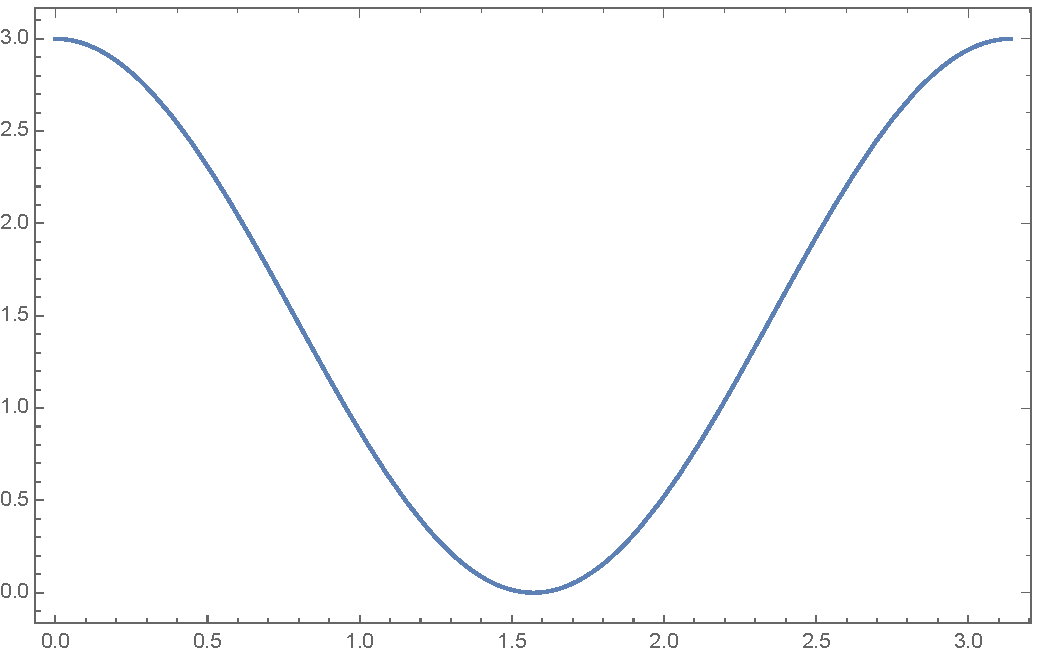
\includegraphics[width=0.8\linewidth]{pol.pdf}
\end{center}
\section*{23.) Field-Free Alignment of Molecules Using Laser Pulses}

We're given the following wave function for $N_2$, at $t=0$;  
$\Psi(\theta,\phi,t=0)=\frac{1}{\sqrt{11}}\sum_{J=0}^{10}Y_J^{m=0}(\theta,\phi)e^{iJ\pi/4}$\\

\textbf{a)} At $J=0$, the expectation value $\braket{cos^2\theta}$ is calculated by first normalizing the wavefunction;\\

${\displaystyle\int_0^\pi}sin\theta d\theta{\displaystyle\int_0^{2\pi}}d\phi\Psi_{J=0}^*\Psi_{J=0}={\displaystyle\int_0^\pi}sin\theta d\theta{\displaystyle\int_0^{2\pi}}d\phi(\frac{1}{\sqrt{11}}\frac{1}{\sqrt{4\pi}})(\frac{1}{\sqrt{11}}\frac{1}{\sqrt{4\pi}})=\frac{1}{11}\frac{1}{4\pi}(2)(2\pi)=\frac{1}{11}$\\

Next;
${\displaystyle\int_0^\pi}sin\theta d\theta{\displaystyle\int_0^{2\pi}}d\phi\Psi_{J=0}^*cos^2\theta\Psi_{J=0}=\frac{1}{11}\frac{1}{4\pi}(2\pi){\displaystyle\int_0^{\pi}}sin\theta cos^2\theta d\theta=\frac{1}{11}\frac{1}{4\pi}(2\pi)(\frac{2}{3})=\frac{1}{33}$\\

Now, dividing by the first result; $\frac{1}{33}/\frac{1}{11}=\frac{1}{3}$\\

A word on part \textbf{b)} and \textbf{c)};\\

I could not for the life of me figure out these questions in the time allotted, but will be working on them independently.
\end{document}
